% Optional replacement caption for the EXISTING Figure 2; the PNG is unchanged.
% Requires graphicx. Paths are relative to the repository root.
\begin{figure}[htbp]
\centering
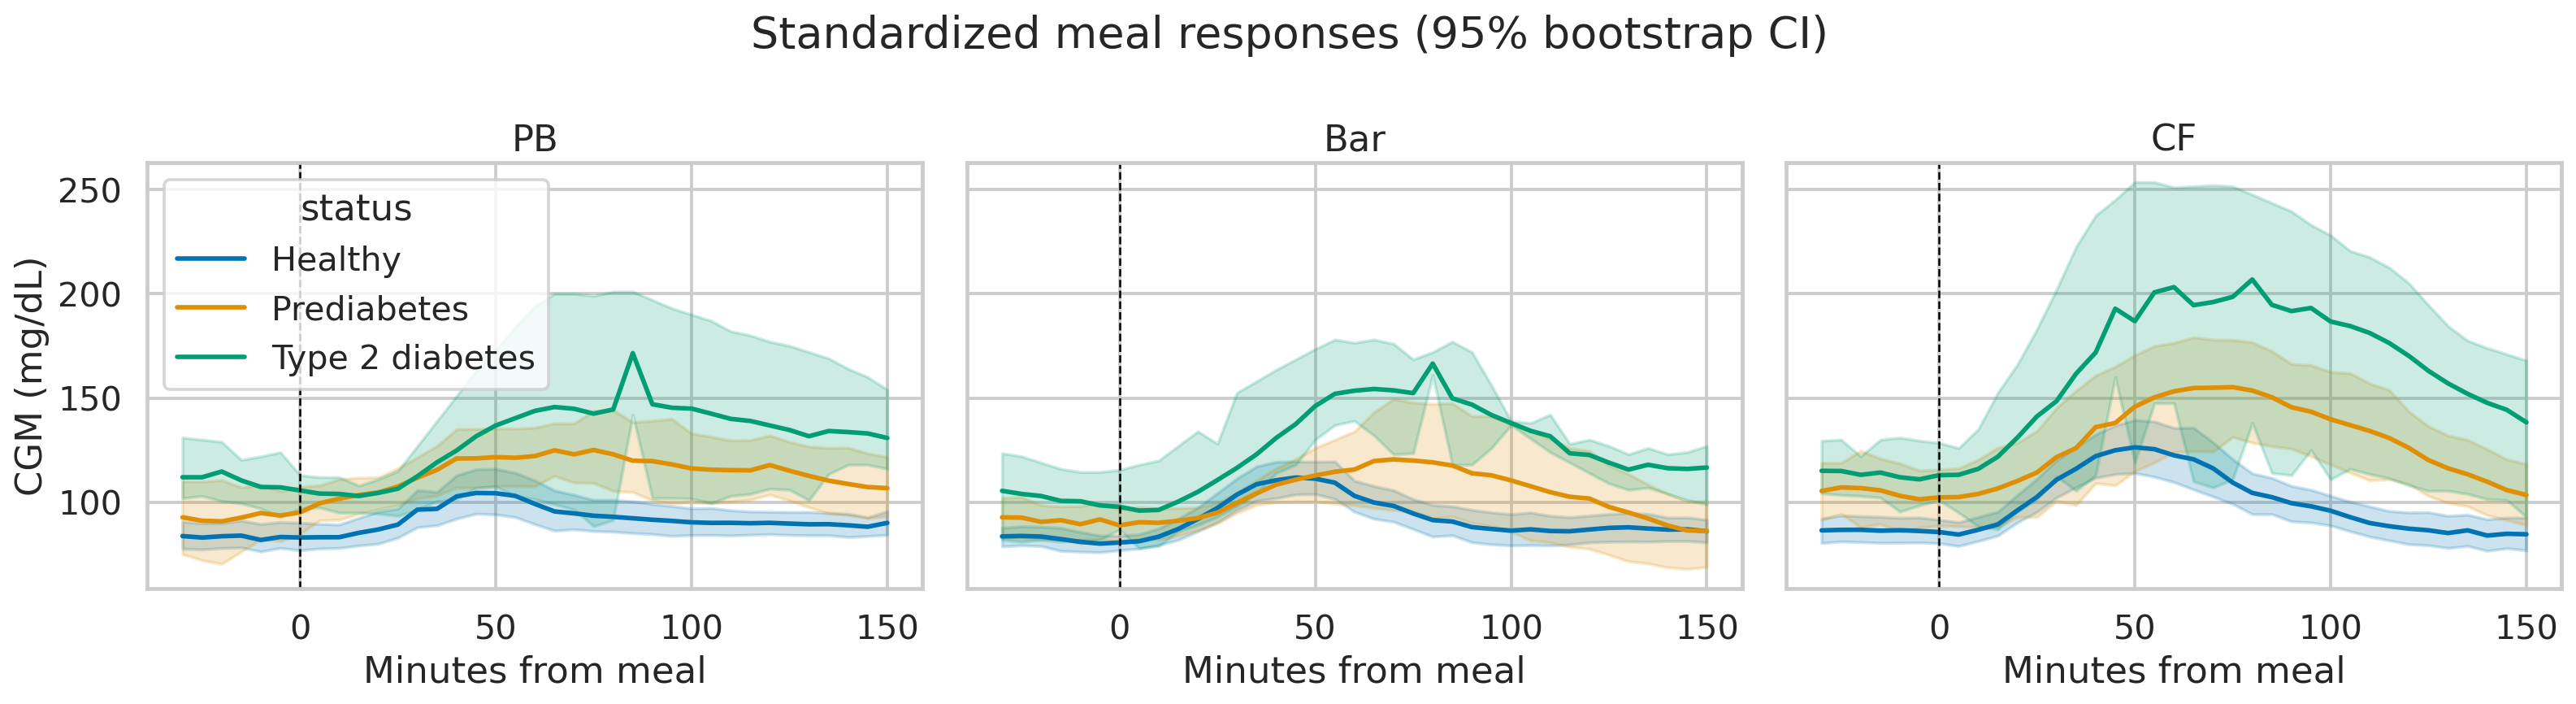
\includegraphics[width=\linewidth]{outputs/figures/figure_2_meal_profiles.png}
\caption{Observed CGM profiles around standardized meals in the retained
meal subset. Panels show bread with peanut butter (PB), a protein bar
(Bar), and cornflakes with milk (CF). Time zero (dashed vertical line)
denotes meal onset; glucose is shown in absolute mg/dL. At each relative
time, available repetitions are averaged within a participant before
averaging across participants of the same clinical-status group.
Shaded bands are pointwise 95\% bootstrap confidence intervals for the
group mean, not individual-response or simultaneous confidence bands.
For PB, Bar, and CF respectively, contributing participant/window totals
are 20/36, 20/32, and 19/33 in the Healthy group; 7/11, 7/11, and 7/10
in prediabetes; and 3/4, 3/4, and 3/6 in type 2 diabetes. Pointwise
participant counts may be smaller because of missing samples. Curves
reflect both starting-glucose differences and meal-associated excursions.
These descriptive profiles are observed data, not fitted or controlled
trajectories; the small type 2 diabetes subgroup precludes strong
population-level inference.}
\label{fig:observed-meal-profiles}
\end{figure}
